\documentclass[12pt]{article}
\usepackage[utf8]{inputenc}
\usepackage{geometry}
\usepackage{graphicx}
\usepackage{url} 
\usepackage[bookmarks, colorlinks=false, pdfborder={0 0 0}, pdftitle={<pdf title here>}, pdfauthor={<author's name here>}, pdfsubject={<subject here>}, pdfkeywords={<keywords here>}]{hyperref} 

% \usepackage{amsmath}
% \usepackage{amsfonts}
% \usepackage{amsthm}
% \usepackage{amssymb}

% \usepackage{hyperref}
\usepackage{enumitem}
% \usepackage{float}
% \usepackage{pdfpages}

% \usepackage{alltt}
% \usepackage{xparse}

\usepackage[newfloat]{minted}
% \usepackage{booktabs}
% \usepackage{color, colortbl}

\usepackage{blindtext}

\usepackage{indentfirst}
\usepackage{setspace}

\usepackage{copyrightbox}
\usepackage{url}

% \definecolor{ex}{rgb}{1.00,0.65,0.00}
% \definecolor{bg}{rgb}{0.95,0.95,0.95}
% \setminted
% {
% 	mathescape=true,
% 	xleftmargin=\parindent,
% 	bgcolor=bg,
% 	escapeinside=@@
% }

% \SetupFloatingEnvironment{listing}{name=Code}

\geometry{
  a4paper
}

\newcommand{\titleItem}[2]{
  \large{
    \textbf{#1}
  } \\
  \large{
    #2
  } \\
  \vspace{8pt}
}

\begin{document}

% Cover page
\begin{titlepage}
  \begin{center}

  % Main title
  \begin{figure}[ht]
    \begin{minipage}[l]{.09\textwidth}
      
\includegraphics[width=\linewidth]{img/metu-logo.png}
    \end{minipage}
    \begin{minipage}[c]{.8\textwidth}
      \centering
      \large{
        \textbf{MIDDLE EAST TECHNICAL UNIVERSITY}
      }

      \normalsize{
        \textbf{DEPARTMENT OF COMPUTER ENGINEERING}
      }
    \end{minipage}
    \begin{minipage}[r]{.09\textwidth}
      
\includegraphics[width=\linewidth]{img/metu-ceng-logo.png}
    \end{minipage}
  \end{figure}
  
  % Course Code
  \vspace{16pt}
  \large{
    \textbf{SUMMER PRACTICE REPORT}
  } \\
  \large{
    \textbf{CENG 300}
  }

  % Submitted by
  \vspace{48pt}
  \titleItem{STUDENT NAME}{Burak Metehan Tunçel}
  \titleItem{ORGANIZATION NAME}{OBSS Teknoloji A.Ş.}
    \vspace{-8pt}
    \begin{figure}[ht]
      \centering
      
\includegraphics[]{img/obss-logo.png}
    \end{figure}
  \titleItem{ADDRESS}{Teknopark İstanbul Sanayi Mah. Teknopark Bulvarı Blok:8A Kat No:3 34906 Pendik/İstanbul 
  }
  \titleItem{DATE}{18.07.2022 - 26.08.2022}
  \titleItem{TOTAL WORKING DAYS}{30}

  % Signature
  \vspace{24pt}
  \begin{minipage}{.49\textwidth}
    \centering
    \normalsize{
      \textbf{STUDENT'S SIGNATURE}
    }
  \end{minipage}
  \begin{minipage}{.49\textwidth}
    \centering
    \normalsize{
      \textbf{ORGANIZATION APPROVAL}
    }
  \end{minipage}

  \end{center}
\end{titlepage}
  

\tableofcontents
\newpage

\onehalfspacing

% Introduction and Information About Company
\section{Introduction}

I have done my first summer practice at OBSS as a software engineer intern for 30 working days between the above dates. Since the intern programs of the OBSS are remote and my department accepts remote practices, I have done the practice online/remotely.

I had an informative internship and learned a lot in Java and web development. My internship included two parts: knowledge sharing and developing a project. In the first part, knowledge about Java and web development were shared, while in the second part, I focused on developing a project with the knowledge I had acquired in the early weeks in practice.

In this report, I will express what I have learned and my experiences in practice at OBSS.

\section{About Company}

OBSS is a company established in 2005 as a software and consulting company, and today, it is one of Turkey's most powerful corporate technology consulting companies. The company has three offices located in İstanbul, Ankara, and Amsterdam. OBSS is the first and the leading Atlassian Partner in Turkey.

From software architecture to coding, from application development to analysis and software testing, the company tries to include all interactive areas of corporate technology in its service range with the aim of providing the most appropriate solutions to its customers.

OBSS has 6+ different internship programs with 100+ interns every year. OBSS shares in 5+ broad expertise sectors with 17+ years of sector experience. 750+ people work at OBSS, and they have built 700+ projects. Additionally, OBSS has several spin-off products and companies. Two of them are Witwiser, which focuses on online assessment solutions and products in international markets, and intouch, a flexible mobile application to meet communities' communication and interaction needs.


% First Week
\section{First Week: Core of Java}


\subsection{Orientation}

On the first day of my internship, the company introduced itself by 1-hour orientation. The orientation provided general information about the company and internship programs. Information about management systems, personal data protection law (KVKK), and occupational health and safety (OHS) are also given.

After the orientation, I met with my team. Firstly, our mentor introduced himself, and then everyone did so. The general internship schedule was shared, and our responsibilities in our internship were stated. Our primary responsibility was to attend the programs/classes on time.


\subsection{Environment Setup and First Program}

Since we have been using Java during our internship, necessary development environments should be introduced and installed. After the setup of Java SDK was shown, we discussed the coding environment. Our mentor suggested IntelliJ IDEA and led its installation.

After we discussed what software is and how it works on a computer and programming languages, we talked about Java's history and working structure. Then, we continued by creating the first project on IntelliJ IDEA, and we coded the first program, the classic \textit{Hello World!}.


\subsection{Introduction to Java}

We started with the basics learned/taught while ordinarily learning a new programming language. The first week's four days were about Java's basics and core concepts. Since syntax and basic concepts of Java are pretty similar to C and C++, understanding the topics was not that hard for me at the beginning of the week. Even though I was learning some tricks about Java and coding, generally, it was like I was learning the syntax of Java.

While learning the concepts and basics, we usually practiced them. The usual process was that after we first coded the exercise, we examined the sample solutions other team members coded. If there was an error in someone's code or someone could not understand a part of the example, we learned by looking at those codes together. This approach has been constructive for me at times because examining the codes of other people helps the learning phase.

\subsubsection{Basics of Java}

We talked about comments, identifiers, escape sequences, data types, operators, basic input and output, conditions, and loops. While learning these, data types were, most probably, the most complicated part. Although I was familiar with the terms ``call-by-value'' or ``call-by-reference'', I believe that to gain a deep understanding of data types in Java language, the time needed to be devoted to them. Strings in Java, for example, can be considered as both primitive and reference data types.

Then, arrays whose preferred syntax in Java is different than C++, type casting, and variable length argument lists came up. Arrays and type casting work almost identically in both Java and C++. Even though other programming languages include that, it was the first time I heard of the ``variable length argument lists'', which are used for an unspecified number of arguments.

Strings have special positions in some languages, and I believe Java is one of them. Strings can be confused because they can behave like both primitive and reference types. Also, I learned about \textit{StringBuffer} and \textit{StringBuilder}, which are basic classes to construct strings and add some functionality to them. Even though I knew what exceptions were, I did not practice much. In fact, I can say that I learned how it works and its actual use in this internship.

We also talked about advanced Java IO as well as the concept of ``serialization'',  the conversion of the state of an object into a byte stream. I believe that although it is a little bit harder than other languages I use, such as Python, file handling is a little bit more flexible in Java, thanks to variety. There are several classes to make file reading and writing easier.

After these basics, some advanced features such as enumerations, interfaces, abstract, and generic classes are discussed. Although these were not new to me, I barely knew what they were and why we use them, but thanks to the exercises, I understood these. Interfaces were a little bit tricky for me because it was the first time I had encountered such a thing. Then, an unfamiliar topic arose: wildcards about which I did not know anything but practical.

\subsubsection{Collections in Java}

From the courses I have taken, I know some data structures. In this part, I learned that Java provides a variety of collections whose implementations are different under the hood. The collections that are in the figure below are discussed.  

% Taken from https://facingissuesonit.com/2019/10/15/java-collection-framework-hierarchy/
\begin{figure}[h!]
  \centering
  \copyrightbox[b]{
    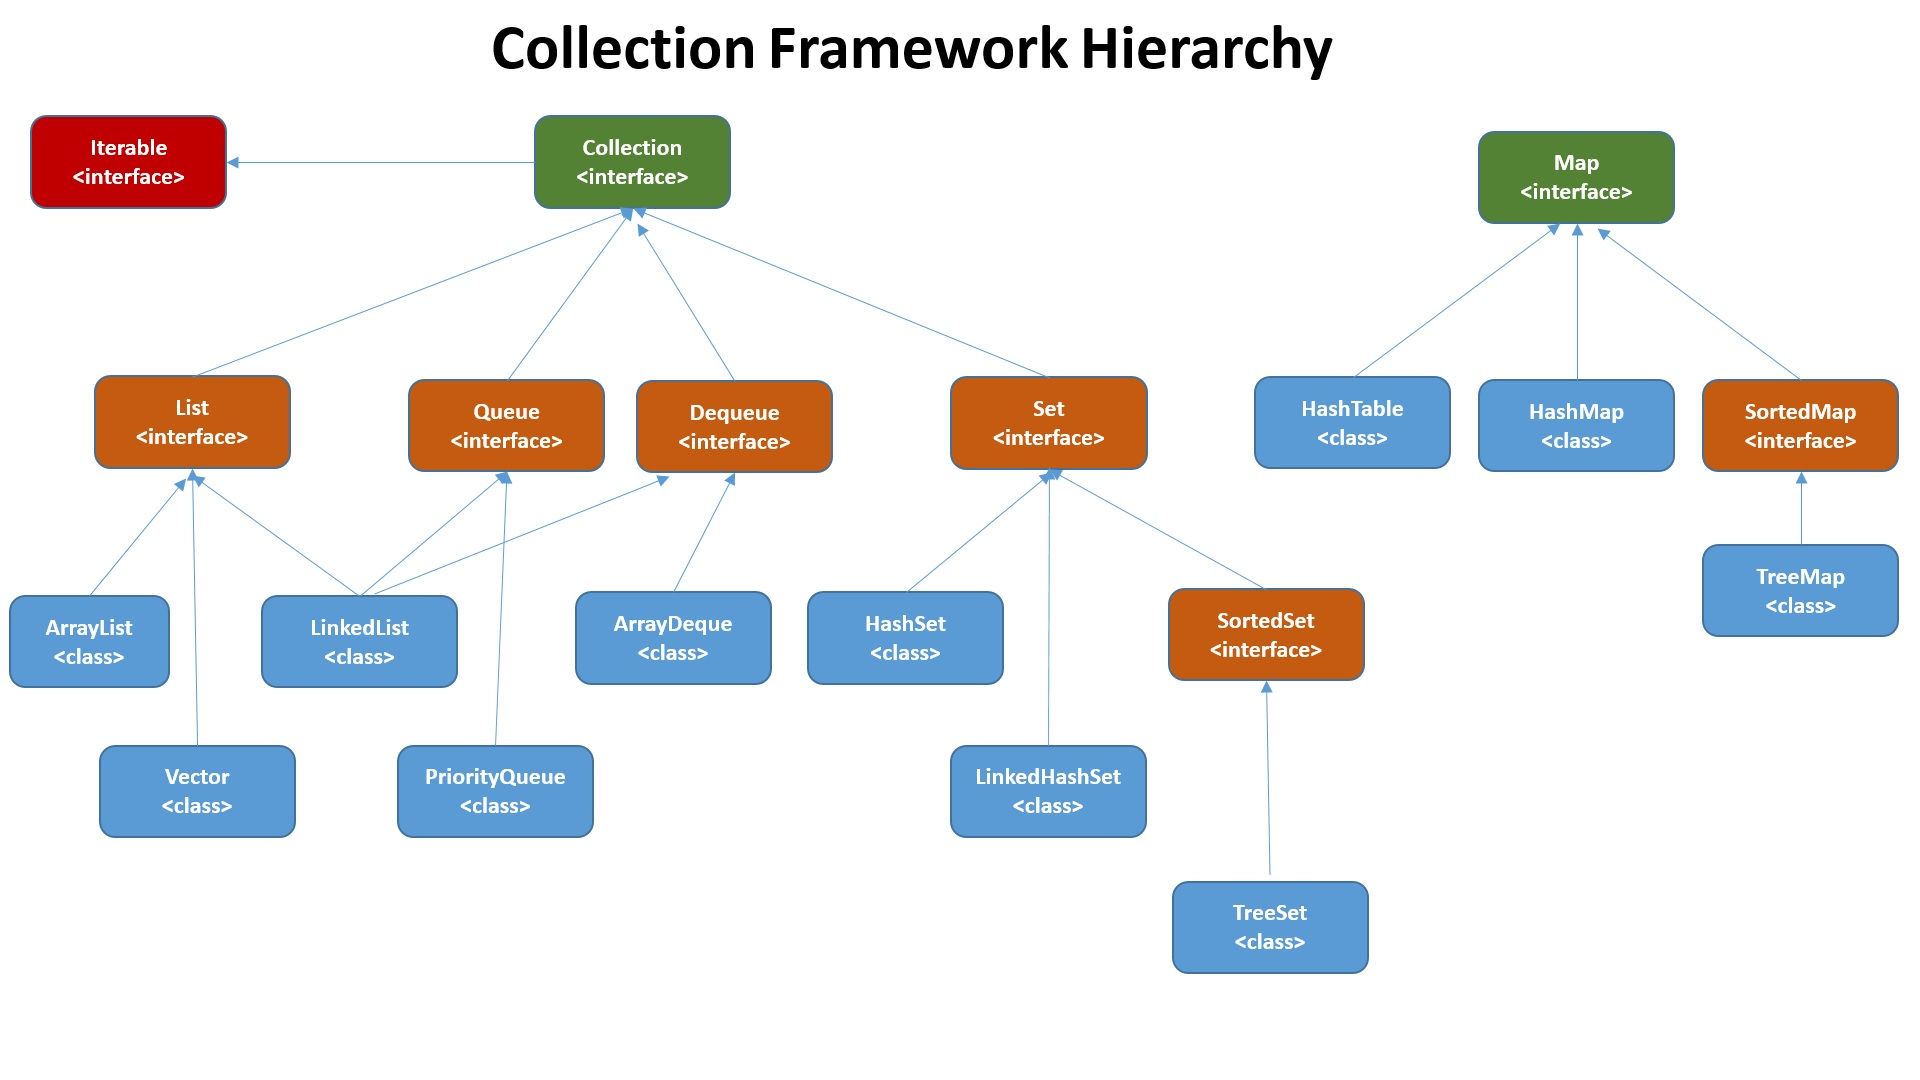
\includegraphics[width=\linewidth]{img/java-collection.jpg}
  }{
    Source: \url{https://facingissuesonit.com/2019/10/15/java-collection-framework-hierarchy/}
  }
\end{figure}

Also, \texttt{hashCode()} and \texttt{equals()}, important methods for these collections to work properly, were discussed. It was shown what they are and why we use them.

\subsubsection{OOP}

This part covered the basics and principles of Object Oriented Programming (OOP).

We started by discussing the basics, such as scopes, constructors, access modifiers, setter and getter methods, method overloading, and static methods. Since I was familiar with concepts from the CENG 242: Programming Language Concepts, I did not have a hard time with these concepts.

After the basics, we moved into the principles. We started with inheritance and class hierarchy. Here, I learned what superclasses and subclasses are and that Java does not support multiple inheritances. Furthermore, behaviors of some concepts, such as access modifiers and constructors, in inheritance are discussed. Also, other principles of abstraction, encapsulation, and polymorphism are covered, but I did not learn new information.

\subsubsection{JavaBeans and JDBC}

The last day of the week, when we got out of the basics of Java and learned databases and database connections by using Java, was a day that I learned new information and was challenged for the first time this week.

We started by talking the JavaBeans, which is a standard. By learning and reading about JavaBeans, I realized that many things are standardized in Java, and implementations are competed instead of the standards. This makes the reason why Java is exceptionally preferred in corporate areas clear.

Since we would have needed to add some dependencies and Maven would be used in our projects, we talked about Maven, a build automation tool, and installed it in addition to MySQL, which was going to be used as a database. After the installations and the environment adjustments, we dived into the Java Database Connectivity (JDBC), Java API that mainly manages connecting to a database. Connecting to a database, executing queries, using of ``\texttt{Statement}'', ``\texttt{ResultSet}'' and ``\texttt{PreparedStatement}'' which are basically used to sending SQL statements to databases, and transaction management.


\subsection{Git \& Bitbucket}

To our use during the internship, we were provided a Bitbucket account. We were asked to use Git and ``\textit{push}'' our codes to Bitbucket. Since we were asked to use Git, the basics and primary usage of Git and Bitbucket were shown. 


% \noindent Additionally, the OOP examples are done:
% \begin{itemize}
%   \item \textbf{ExampleThePen:} Constructors, Set and Get methods, Shadowing, \texttt{static} keyword.
%   \item \textbf{ExampleBusReservation:} Constructors, Set and Get methods, Shadowing, \texttt{static} keyword, Enumerations.
% \end{itemize}

% Example of the topic: \texttt{ExampleException}, Example IO

% The example \texttt{ExampleOccurrencesOfWords} is done.

% Some days, Some friends was talking about design patterns. In the third day of my internship, two people talked about two different design patterns, which are \textit{Adepter} and \textit{MVC} design patterns.

% New projects are opened after Inner Class part: \texttt{JIP-JDBC}.

% After these concepts are disccussed, example named \texttt{ExamplePenRevisited} is done.

% We have done the example named \texttt{ExampleInterfacePen}.

\end{document}